\documentclass[11pt]{article}
\usepackage{graphicx}
\usepackage[T1]{fontenc}
\usepackage{txfonts}
\setcounter{secnumdepth}{0}
\usepackage[affil-it]{authblk}   % author affiliation
\usepackage{lineno} %line numbers
\usepackage[a4paper, total={6.5in, 8.5in}]{geometry} % set page size
\usepackage{setspace}
\doublespacing


\begin{document}

\title{Demographic Bias in Human Cell Studies }
\author{Jessica Snyder\textsuperscript{1}, Iva Bojic\textsuperscript{1,2}, Aarom Gerow\textsuperscript{3}, Carlo Ratti  \textsuperscript{1,2 } \\ \textsuperscript{1}Massachusetts Institute of Technology, SENSEable City Lab \\ \textsuperscript{2}Singapore-MIT Alliance for Research and Technology \\  \textsuperscript{3}The University of Chicago, Knowledge Lab }

\maketitle

\section{Abstract}
Health research has standardized breast cancer models, using a handful of cell lines, which has successfully generated survival rates near 90\%, while failing to balance the demographics, and consequently tumor sub-types, of the patient population, possibly contributing to increased morbidity among demographic not represented in the most heavily used cell lines. Re-evaluating the use of cell lines are used to improve breast cancer treatment options, for a broader range of tumor sub-types, begins with a data-driven analysis of which and how cell lines have been used in published research and patents. 

\section{Rationale}

An estimated \$150 billion USD will be spent from 2010-2020 on nearly 20 million cancer patients \cite{mariotto2011projections}. The most common cancer in women, second overall to prostate cancer, is breast cancer, comprising 32\% of the cost \cite{mariotto2011projections}. Breast cancer statistics published by the Center for Disease Control (CDC) since 1999 show that while white woman are more likely to develop breast cancer, black patients are less likely to survive than other races, exposing a well-acknowledged disparity in the efficacy of breast cancer treatment for black women \cite{greenlee2000cancer, berkman2014racial}. The likely causes include societal, behavioral and biological factors, broadly categorized as extrinsic factors which are the responsibility of public policy and the individual, and intrinsic factors, such as genetics and cell structure within aggressive tumor sub-types, which are the responsibility of medical researchers to consider in designing fundamental research studies \cite{reding2012examination, brennan2012there}. 

Raising the survival rate of black breast cancer patients to the national average requires critical review of socioeconomic-dependence of high-quality health care access and inclusive diagnostic techniques, without question \cite{shavers2003racial}. Failing to diagnosis at early stages, as well as faster growing, more aggressive tumor sub-types, disproportionately effect black patients \cite{batina2013variation}. 

Vetting the influence of intrinsic factors of breast cancer is critical to guide the action of fundamental medical research, especially the types of cell lines used in foundational research. Are there intrinsic factors of the tumor sub-types causing morbidity, which are disproportionately present in in black breast cancer patients? Environmental exposure and genetic background determine the breast cancer's subtypes, aggressiveness, and ultimately, patient's prognosis. Highly aggressive tumor subtypes are correlated to risk factors such as obesity, which disproportionately effects black women. Self-reported race correlated to breast cancer properties, such as estrogen receptor status and stage of diagnosis, more than percent African ancestry, suggesting social determinants shape the disease physiology more than genetic predispositions \cite{reding2012examination}. Currently, alternative treatment options for patients with a genetic predisposition for hormone receptor-negative breast cancers, which are also likely black, is  limited \cite{huo2009population}.

Research supports black breast cancer patients present elevated risk for aggressive, intrinsic factors of breast cancer which adversely effect prognosis. The next logical question is to what extent have black patients donated to cell lines used by medical researchers, and then, how well these lines are represented in published research and patents. The purpose of asking these questions is to determine any extent to under-representation, allowing for corrective action to simply include cell lines which represent the aggressive tumor sub-types causing the most morbidity. Data-driven retrospectives on disease burden and treatment effectiveness have been used in the past to guide medical research funding and health policy decisions towards the most productive population-level outcomes \cite{kim2016cancer}. 

The long term consequences of medical research in demographics most heavily represented as donors to biopsies used in lab work have the best prognosis for treatment. Targeted breast cancer therapies and preventative screening sensitive to various tumors are required to absolve demographic inequalities in breast cancer treatment \cite{batina2013variation}. Cell lines are a critical tool of scientific discovery for medical treatments. ``Human cancer in a test tube'' provides a standard for genotypic and phenotypic stability. 

US CDC statistics publishes statistics on the number of women diagnosed with breast cancer divided by the population size of women multiplied by 100k, for all women and for each ethnicity. Similarly, the death rate is published as a function of the number of woman. White woman are most commonly diagnosed with breast cancer, however black woman are most likely die from the cancer, concluding medical treatment is more effective for white woman than black woman. 

\begin{figure}[h!]
\centering
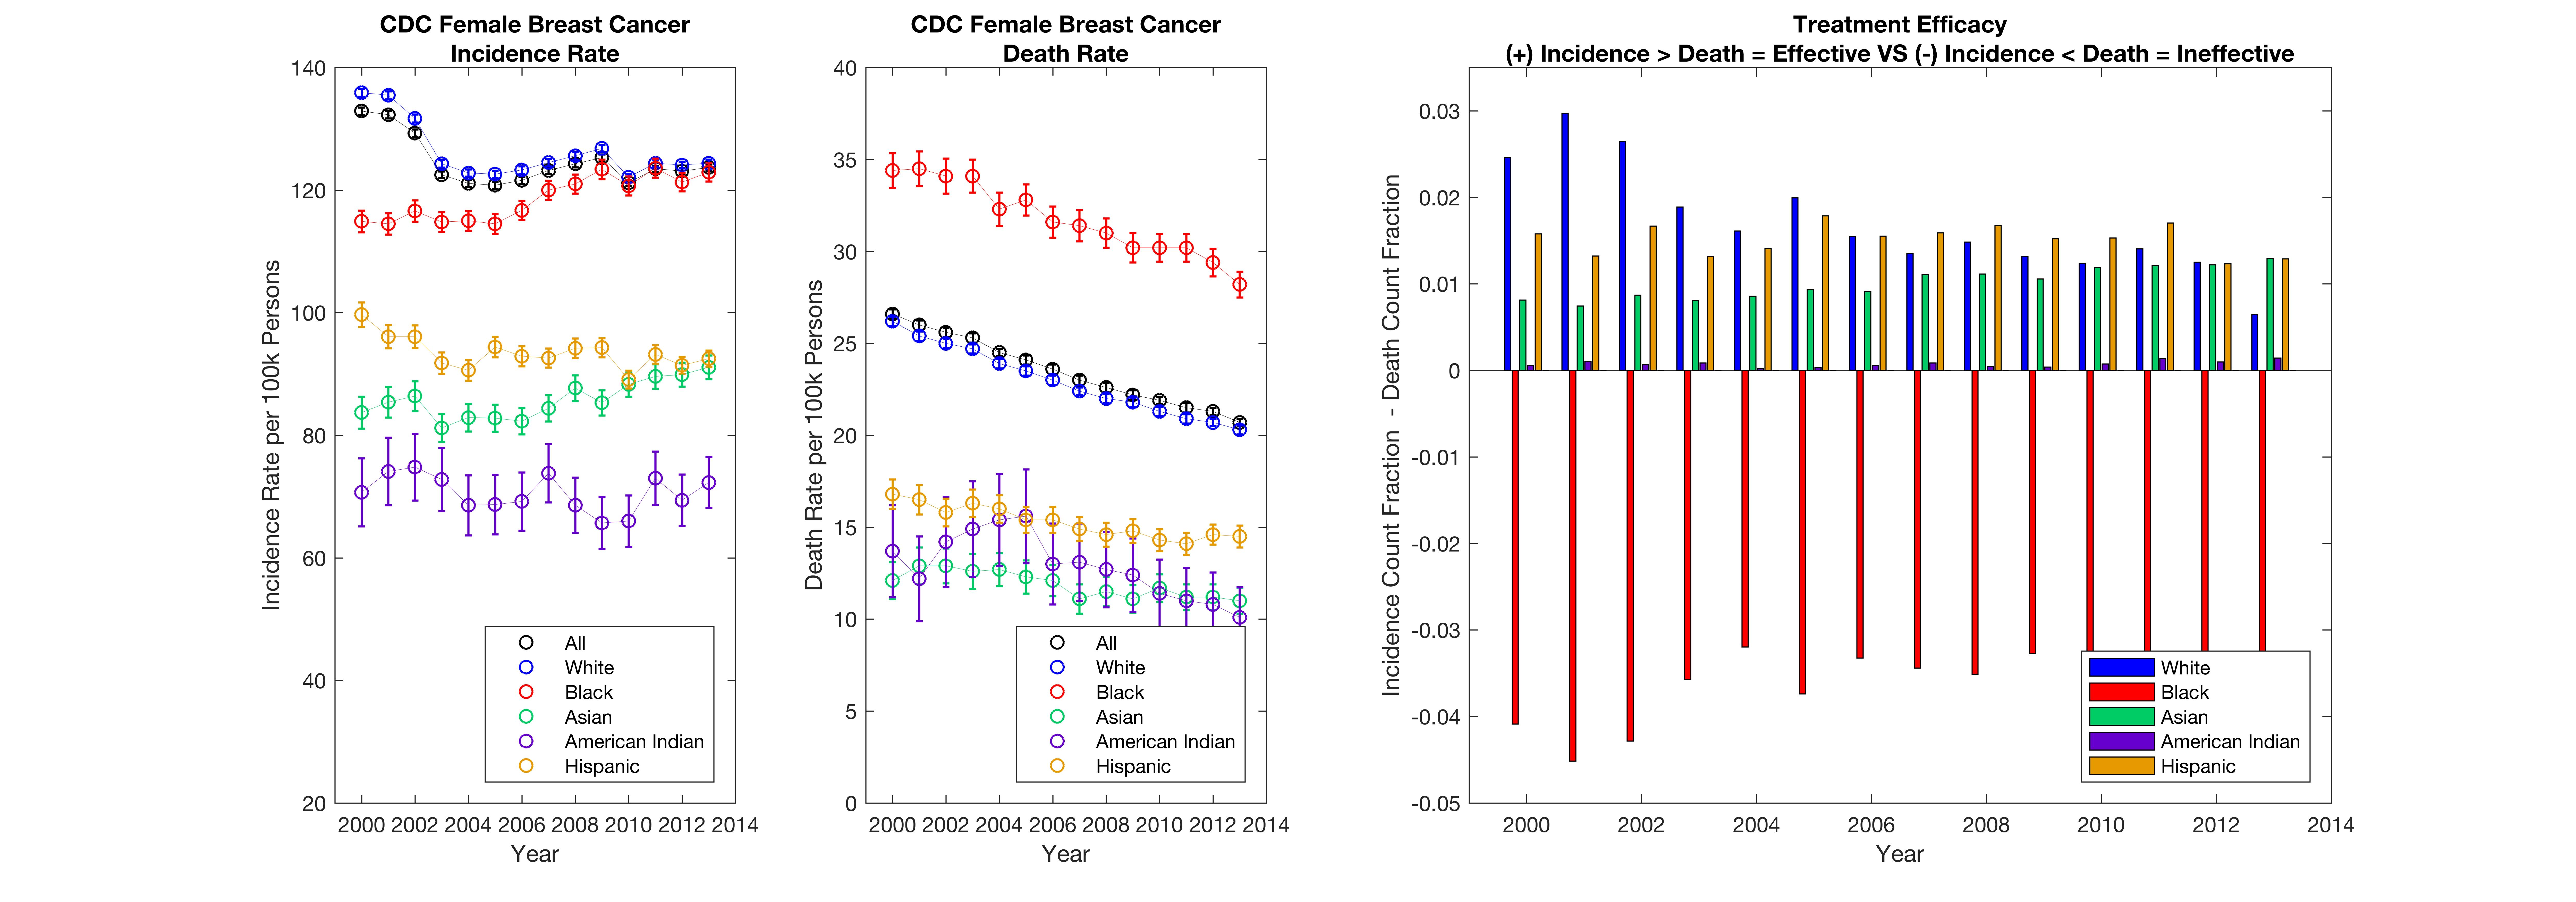
\includegraphics[width=1\columnwidth, trim = {40cm 0cm 30cm 0cm}, clip]{Rationale.jpg}
\caption{\label{PS} Rationale to investigate the representation of cell models derived from black patients in breast cancer research based on a persistent discrepancy in breast cancer treatment efficacy for black patients. }
\end{figure}

\begin{figure}[h!]
\centering
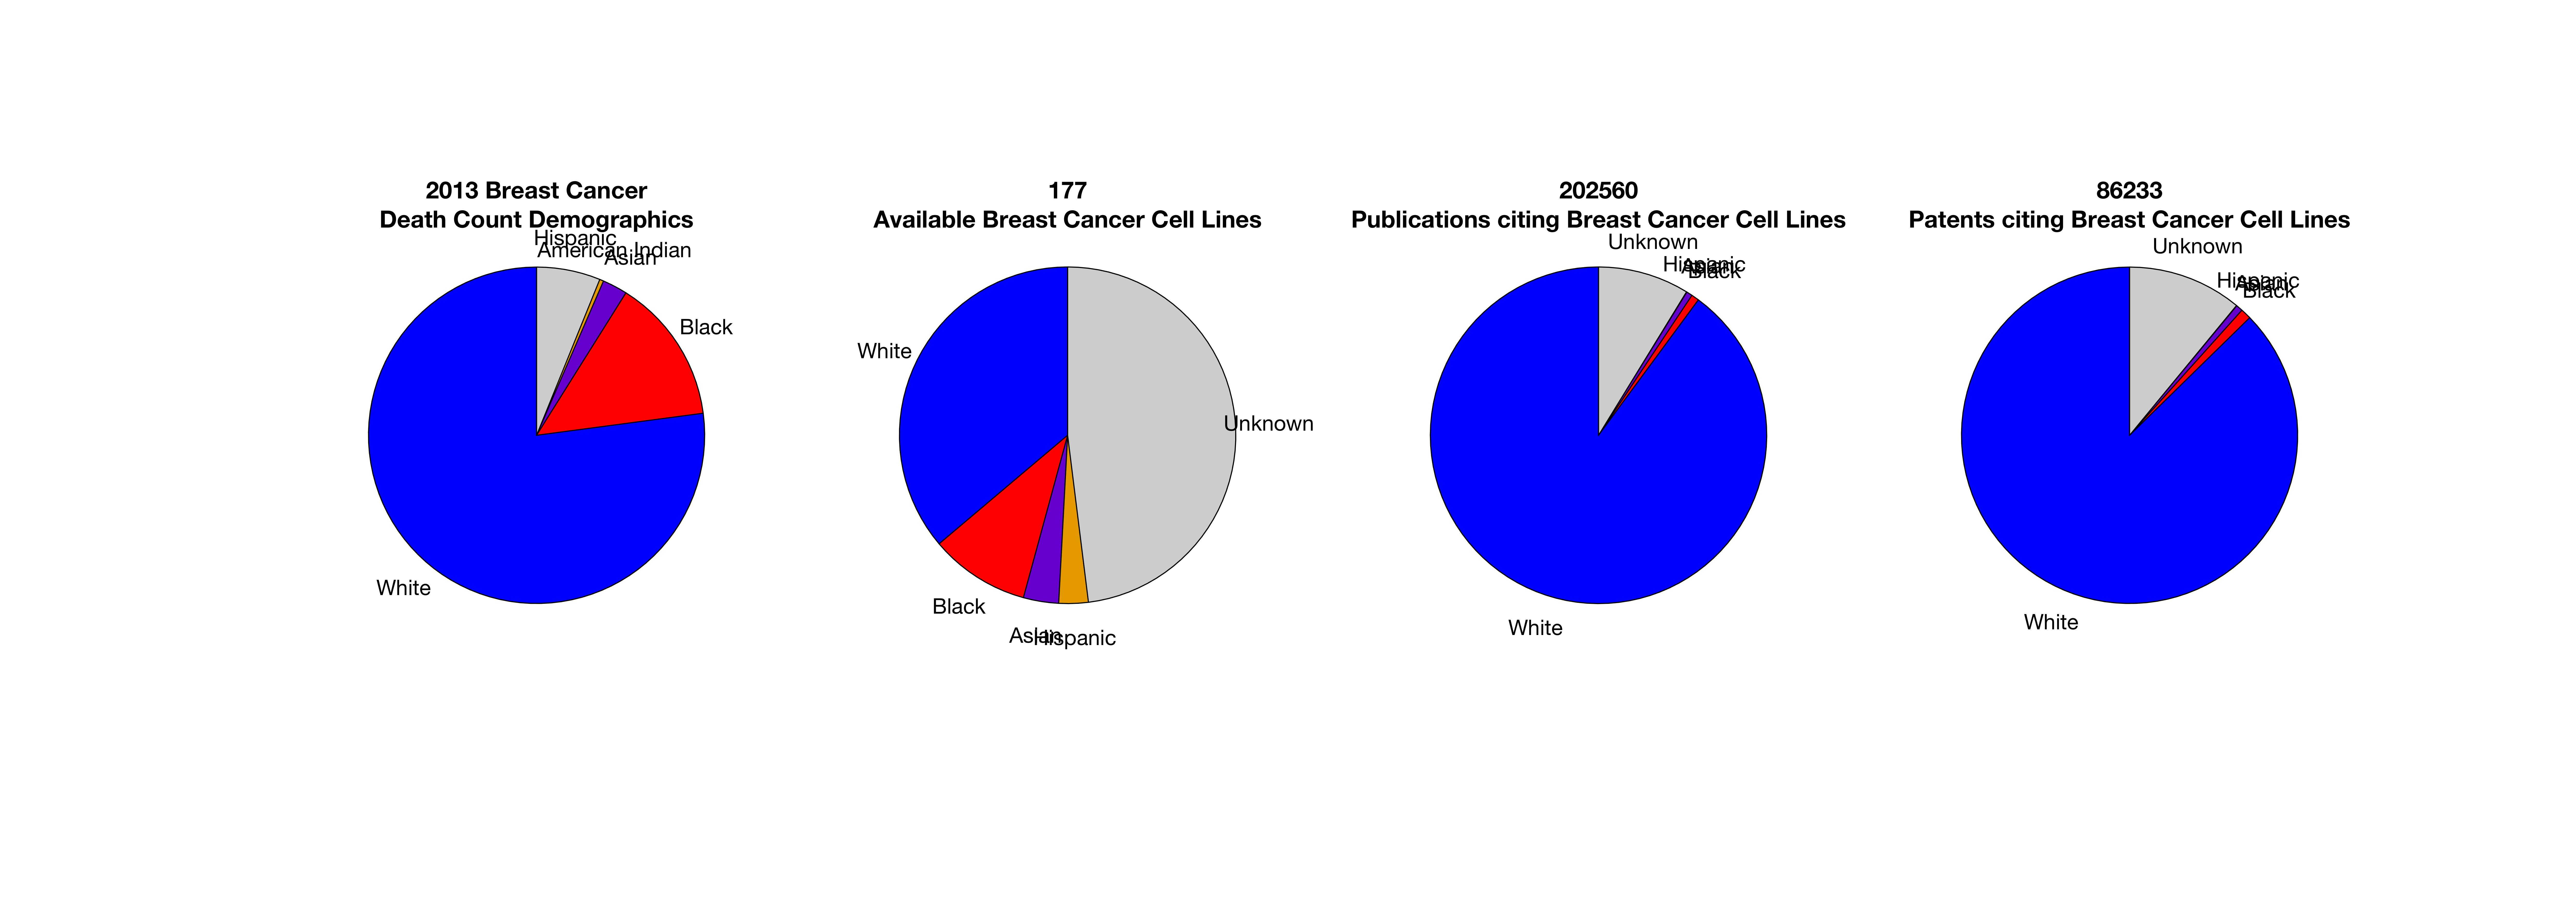
\includegraphics[width=1\columnwidth, trim = {40cm 20cm 30cm 20cm}, clip]{CellLines.jpg}
\caption{\label{PS} Comparison of the need for medical research, as defined by the most recent US CDC breast cancer death counts, to the demographic representation in the available cell models derived from breast tissue, and the use of the available cell lines in publications and US patents.}
\end{figure}

\begin{figure}[h!]
\centering
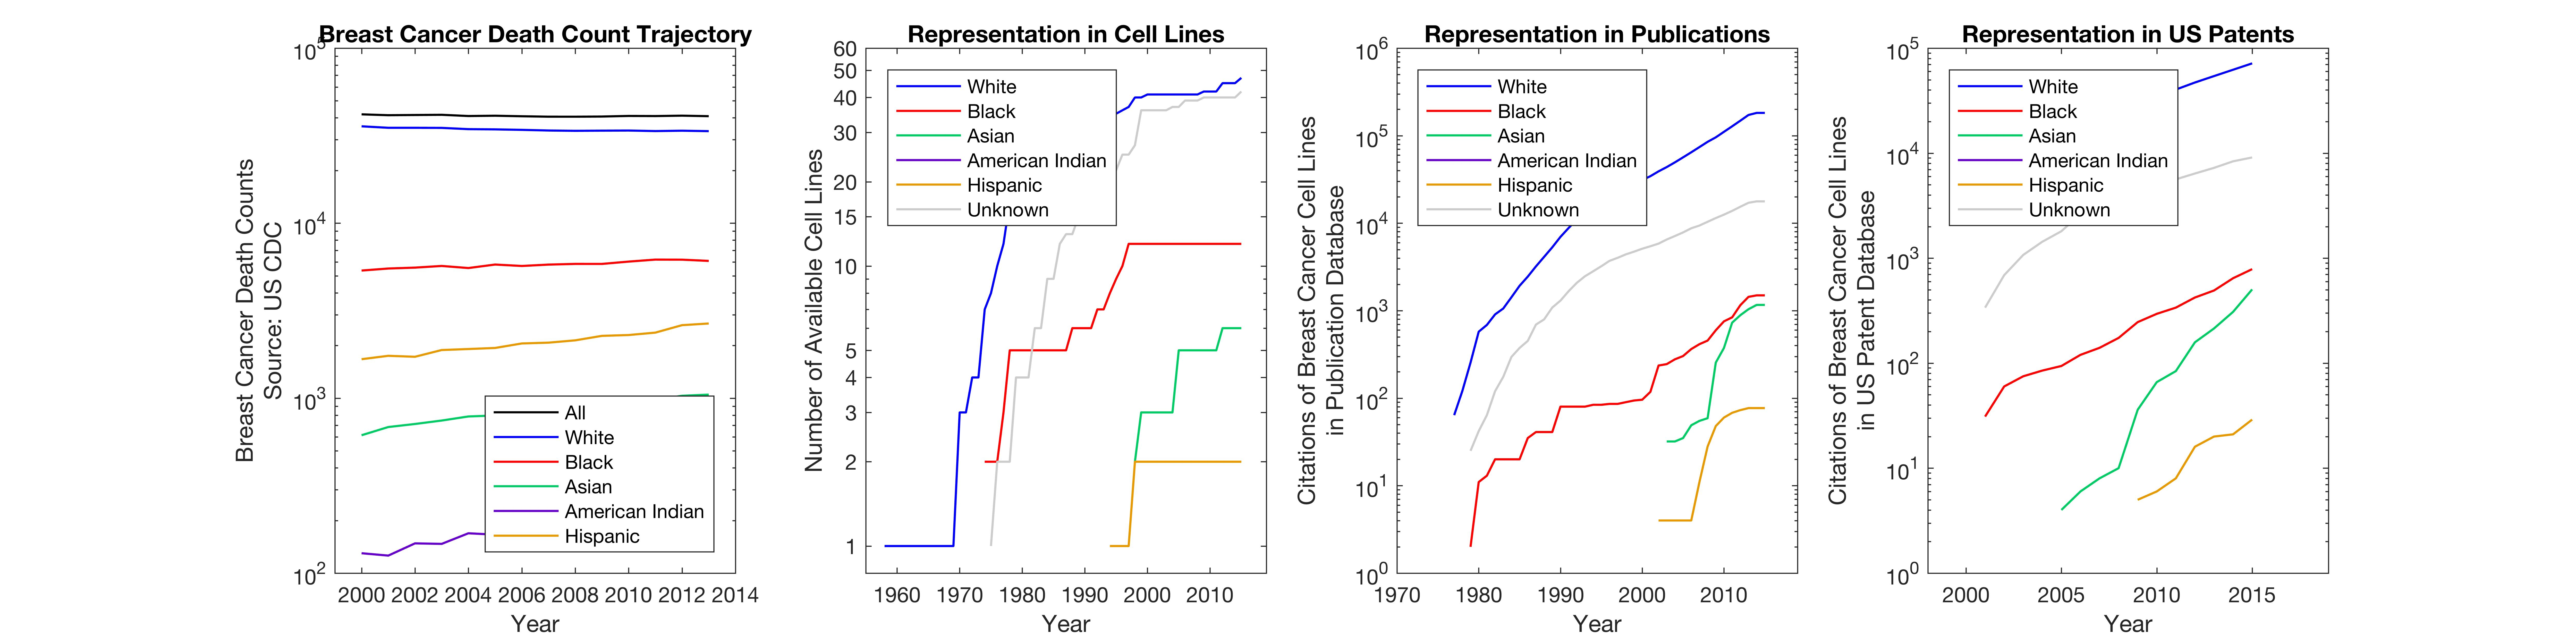
\includegraphics[width=1\columnwidth, trim = {10cm 0cm 10cm 0cm}, clip]{Trajectory.jpg}
\caption{\label{PS} Demographic representation in available cell lines, publication and patents as compared to the death counts for breast cancer.}
\end{figure}

\begin{figure}[h!]
\centering
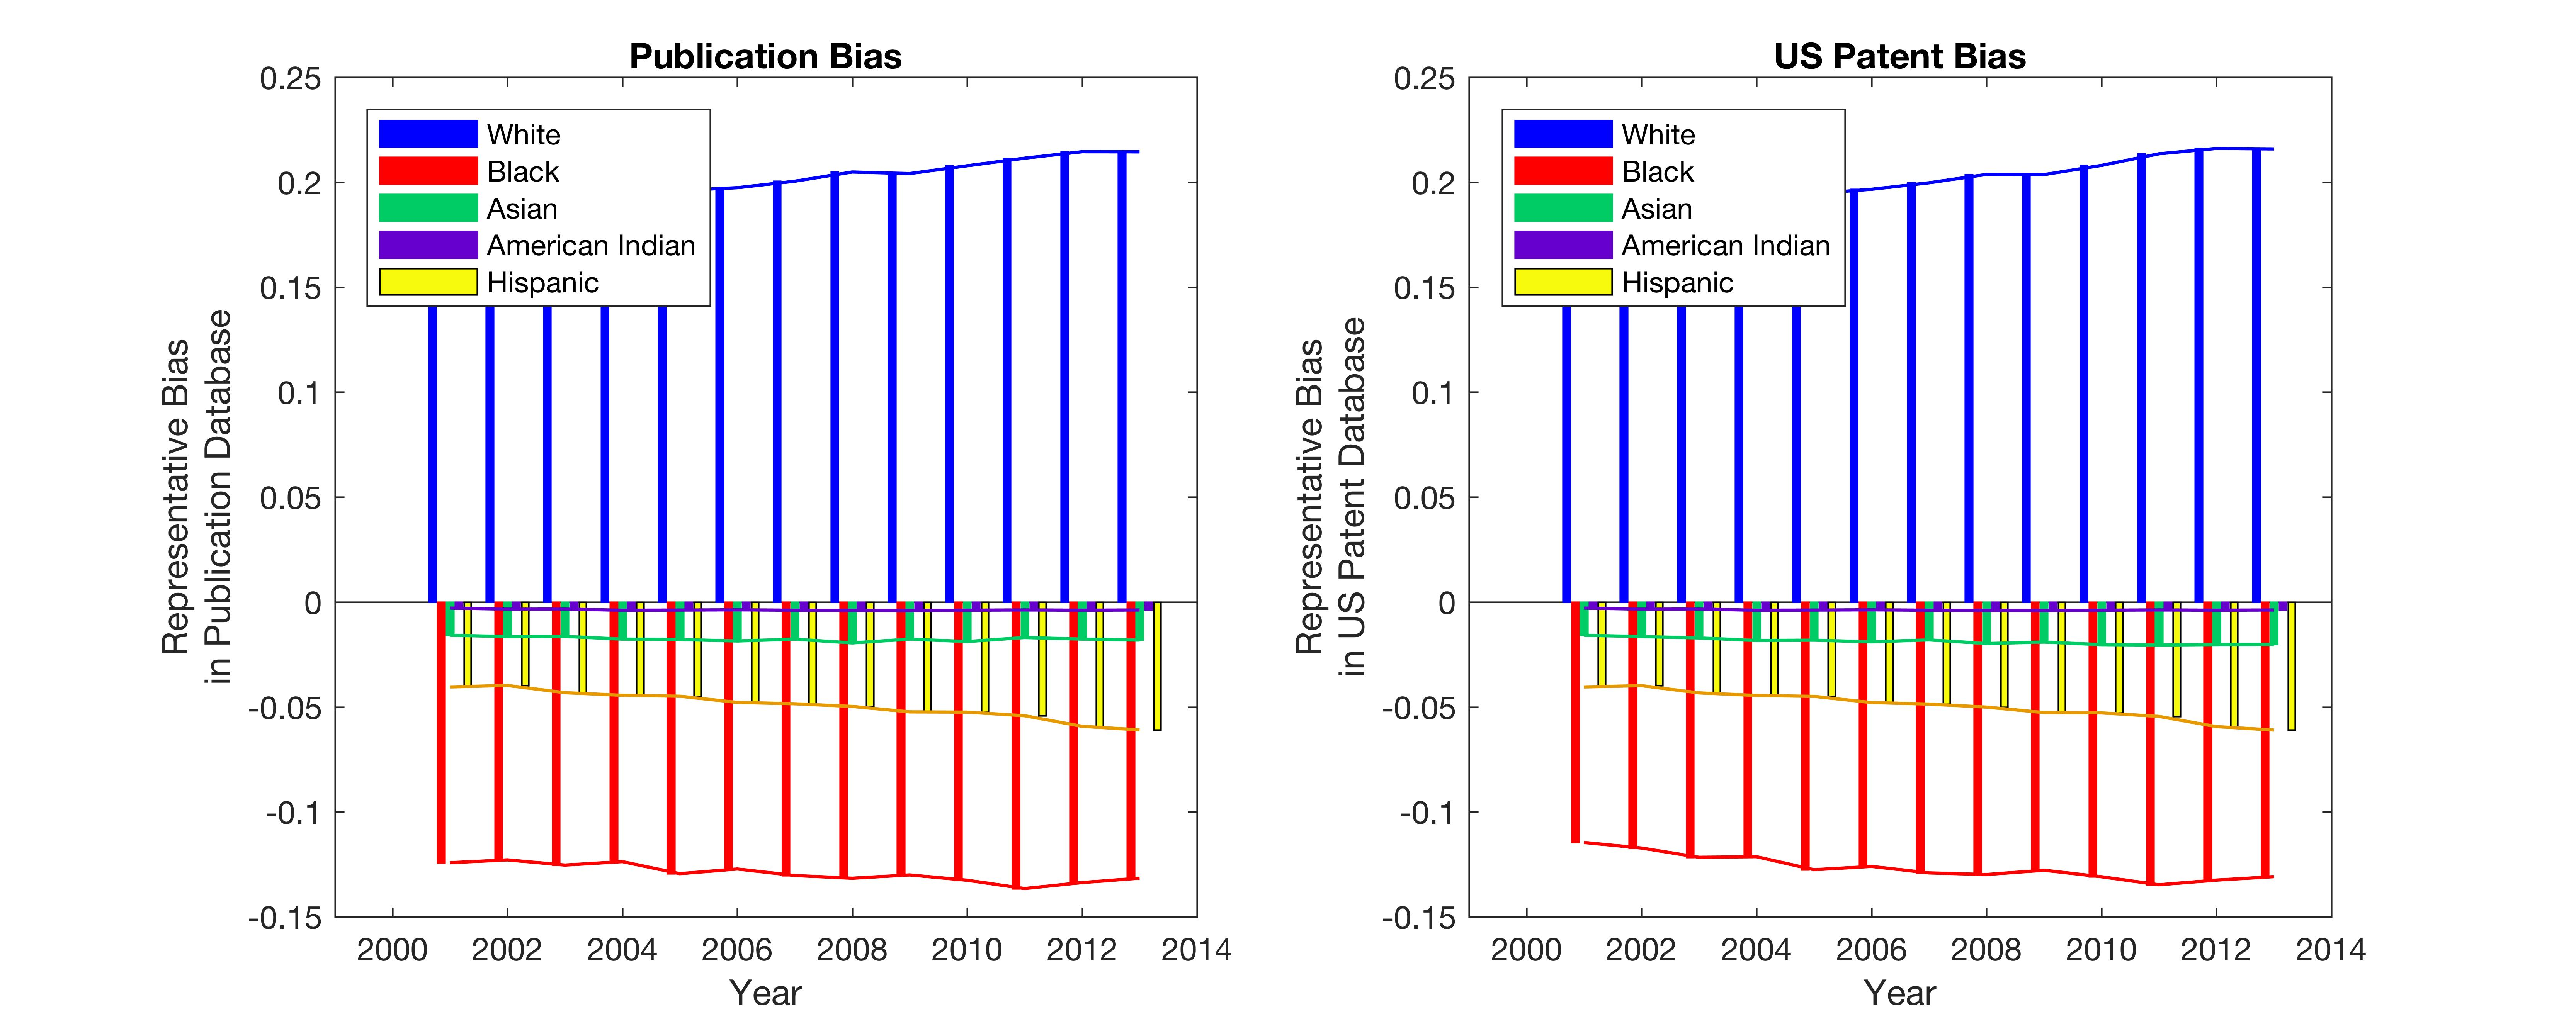
\includegraphics[width=1\columnwidth, trim = {10cm 0cm 10cm 0cm}, clip]{Bias.jpg}
\caption{\label{PS} The representative bias in breast cancer medical research and therapeutic development, as determined by comparing the fraction of each demographic in the breast cancer death count to the number of publications and US patents citing cell lines generated from each ethnicity.}
\end{figure}


\section{The available human cell lines}

 \section{Demographic inclusiveness of the publication record}
 
  \section{Demographic inclusiveness of the US patent database}

\section{Forging ahead with personalized medicine}
Transformative approaches to health care, such as personalized medicine, authenticate the importance of genetic variation on the effectiveness of treatment, physicians use genomic analysis to determine the course of treatment, circumventing the limitations of generalized treatments with tailored treatments. Here, we survey the genetic variation in breast cancer research with human cell models by characterizing the demographics of cell line donors represented in breast cancer research. 

\bibliographystyle{unsrt}
\bibliography{refs}

\section{Methods}

\subsection{Definitions}

\subsection{Cell line nomenclature}

\subsection{Excluding misidentified cell lines}

\subsection{Building the database of publications}

\subsection{Building the database of patents}

\subsection{Comparison to incidence and morbidity counts}

\end{document}